\chapter{Anàlisi amortitzada}

\index{anàlisi amortitzada}

La complexitat temporal d'un algorisme sovint és fàcil d'analitzar
simplement mirant l'estructura de l'algorisme: quins bucles conté
l'algorisme i quantes vegades s'executen. Tanmateix, de
vegades una anàlisi directa no dóna una imatge real de l'eficiència
de l'algorisme.

\key{L'anàlisi amortitzada} es pot fer servir per analitzar algorismes
que contenen operacions la complexitat temporal dels quals varia. La
idea és estimar el temps total utilitzat per totes aquestes
operacions durant l'execució de l'algorisme, en lloc de centrar-se en
les operacions individuals.

\section{Mètode dels dos punters}

\index{mètode dels dos punters}

En el \key{mètode dels dos punters}, es fan servir dos punters per iterar
pels valors d'un vector. Els punters només es poden moure en una
direcció, cosa que garanteix que l'algorisme funciona de manera
eficient. A continuació discutim dos problemes que es poden resoldre
mitjançant el mètode dels dos punters.

\subsubsection{Suma de subvector}

Com a primer exemple, considerem un problema en què se'ns dóna una
vector de $n$ enters positius i una suma objectiu $x$, i volem trobar
un subvector la suma del qual és $x$ o informar que no hi ha aquesta
subvector.

Per exemple, el vector
\begin{center}
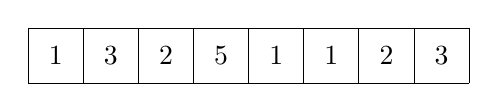
\begin{tikzpicture}[scale=0.7]
\draw (0,0) grid (8,1);

\node at (0.5,0.5) {$1$};
\node at (1.5,0.5) {$3$};
\node at (2.5,0.5) {$2$};
\node at (3.5,0.5) {$5$};
\node at (4.5,0.5) {$1$};
\node at (5.5,0.5) {$1$};
\node at (6.5,0.5) {$2$};
\node at (7.5,0.5) {$3$};
\end{tikzpicture}
\end{center}
conté un subvector la suma del qual és 8:
\begin{center}
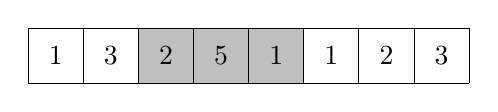
\begin{tikzpicture}[scale=0.7]
\fill[color=lightgray] (2,0) rectangle (5,1);
\draw (0,0) grid (8,1);

\node at (0.5,0.5) {$1$};
\node at (1.5,0.5) {$3$};
\node at (2.5,0.5) {$2$};
\node at (3.5,0.5) {$5$};
\node at (4.5,0.5) {$1$};
\node at (5.5,0.5) {$1$};
\node at (6.5,0.5) {$2$};
\node at (7.5,0.5) {$3$};
\end{tikzpicture}
\end{center}


Aquest problema es pot resoldre en temps $O(n)$ fent servir el mètode
dels dos punters. La idea és mantenir punters que assenyalin el primer
i l'últim valor d'un subvector. En cada gir, el punter esquerre es mou
un pas cap a la dreta i el punter dret es mou cap a la dreta sempre
que la suma del subvector resultant sigui com a màxim $x$. Si la suma
es converteix exactament en $x$, s'ha trobat una solució.

Com a exemple, considereu el vector següent i una suma objectiu $x=8$:
\begin{center}
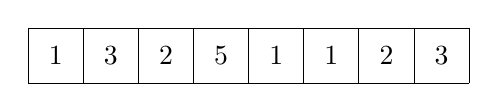
\begin{tikzpicture}[scale=0.7]
\draw (0,0) grid (8,1);

\node at (0.5,0.5) {$1$};
\node at (1.5,0.5) {$3$};
\node at (2.5,0.5) {$2$};
\node at (3.5,0.5) {$5$};
\node at (4.5,0.5) {$1$};
\node at (5.5,0.5) {$1$};
\node at (6.5,0.5) {$2$};
\node at (7.5,0.5) {$3$};
\end{tikzpicture}
\end{center}


El subvector inicial conté els valors 1, 3 i 2 la suma dels quals és 6:


\begin{center}
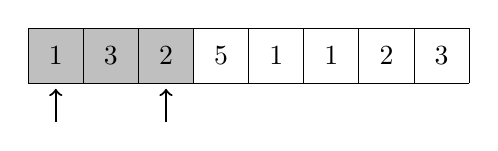
\begin{tikzpicture}[scale=0.7]
\fill[color=lightgray] (0,0) rectangle (3,1);
\draw (0,0) grid (8,1);

\node at (0.5,0.5) {$1$};
\node at (1.5,0.5) {$3$};
\node at (2.5,0.5) {$2$};
\node at (3.5,0.5) {$5$};
\node at (4.5,0.5) {$1$};
\node at (5.5,0.5) {$1$};
\node at (6.5,0.5) {$2$};
\node at (7.5,0.5) {$3$};

\draw[thick,->] (0.5,-0.7) -- (0.5,-0.1);
\draw[thick,->] (2.5,-0.7) -- (2.5,-0.1);
\end{tikzpicture}
\end{center}


Aleshores, el punter esquerre es mou un pas cap a la dreta. El punter
dret no es mou, perquè, en cas contrari, la suma del subvector
superaria $x$.


\begin{center}
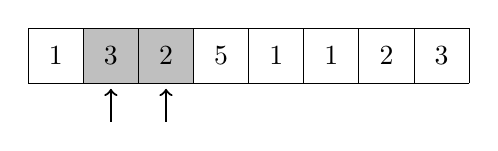
\begin{tikzpicture}[scale=0.7]
\fill[color=lightgray] (1,0) rectangle (3,1);
\draw (0,0) grid (8,1);

\node at (0.5,0.5) {$1$};
\node at (1.5,0.5) {$3$};
\node at (2.5,0.5) {$2$};
\node at (3.5,0.5) {$5$};
\node at (4.5,0.5) {$1$};
\node at (5.5,0.5) {$1$};
\node at (6.5,0.5) {$2$};
\node at (7.5,0.5) {$3$};

\draw[thick,->] (1.5,-0.7) -- (1.5,-0.1);
\draw[thick,->] (2.5,-0.7) -- (2.5,-0.1);
\end{tikzpicture}
\end{center}


De nou, el punter esquerre es mou un pas cap a la dreta, i aquesta
vegada el punter dret es mou tres passos cap a la dreta. La suma del
subvector és $2+5+1=8$, de manera que s'ha trobat un subvector la suma
del qual és $x$.


\begin{center}
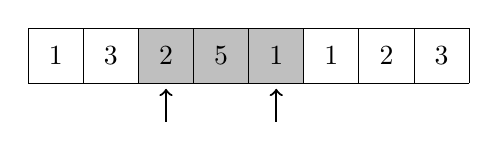
\begin{tikzpicture}[scale=0.7]
\fill[color=lightgray] (2,0) rectangle (5,1);
\draw (0,0) grid (8,1);

\node at (0.5,0.5) {$1$};
\node at (1.5,0.5) {$3$};
\node at (2.5,0.5) {$2$};
\node at (3.5,0.5) {$5$};
\node at (4.5,0.5) {$1$};
\node at (5.5,0.5) {$1$};
\node at (6.5,0.5) {$2$};
\node at (7.5,0.5) {$3$};

\draw[thick,->] (2.5,-0.7) -- (2.5,-0.1);
\draw[thick,->] (4.5,-0.7) -- (4.5,-0.1);
\end{tikzpicture}
\end{center}


El temps d'execució de l'algorisme depèn del nombre de passos que es
mou el punter dret. Tot i que no hi ha cap límit superior útil sobre
quants passos pot moure el punter en un \emph{únic} gir, sabem que el
punter es mou \emph{un total de} $O(n)$ passos durant l'algorisme, perquè
només es mou cap a la dreta.

Com que tant el punter esquerre com el dret es mouen $O(n)$ passos durant
l'algorisme, l'algorisme funciona en el temps $O(n)$.

\subsubsection{Problema 2SUMA}

\index{Problema 2SUMA}

Un altre problema que es pot resoldre mitjançant el mètode dels dos
punters és el següent problema, també conegut com a \key{problema 2SUMA}:
donat un vector de $n$ nombres i una suma objectiu $x$,
trobeu dos valors del vector de manera que suma és $x$, o informeu que
no existeixen aquests valors.

Per resoldre el problema, primer ordenem els valors del vector en
ordre creixent. Després d'això, iterem el vector fent servir dos
punters. El punter esquerre comença al primer valor i es mou un pas
cap a la dreta en cada torn. El punter dret comença a l'últim valor i
sempre es mou cap a l'esquerra fins que la suma del valor esquerre i
dret és com a màxim $x$. Si la suma és exactament $x$, s'ha trobat una
solució.

Per exemple, considereu el vector següent i una suma objectiu $x=12$:
\begin{center}
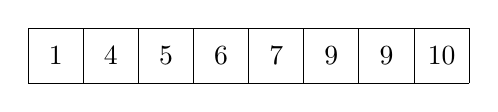
\begin{tikzpicture}[scale=0.7]
\draw (0,0) grid (8,1);

\node at (0.5,0.5) {$1$};
\node at (1.5,0.5) {$4$};
\node at (2.5,0.5) {$5$};
\node at (3.5,0.5) {$6$};
\node at (4.5,0.5) {$7$};
\node at (5.5,0.5) {$9$};
\node at (6.5,0.5) {$9$};
\node at (7.5,0.5) {$10$};
\end{tikzpicture}
\end{center}


Les posicions inicials dels punters són les següents. La suma dels
valors és $1+10=11$ que és més petit que $x$.


\begin{center}
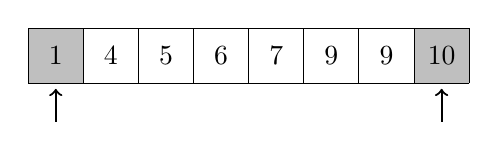
\begin{tikzpicture}[scale=0.7]
\fill[color=lightgray] (0,0) rectangle (1,1);
\fill[color=lightgray] (7,0) rectangle (8,1);
\draw (0,0) grid (8,1);

\node at (0.5,0.5) {$1$};
\node at (1.5,0.5) {$4$};
\node at (2.5,0.5) {$5$};
\node at (3.5,0.5) {$6$};
\node at (4.5,0.5) {$7$};
\node at (5.5,0.5) {$9$};
\node at (6.5,0.5) {$9$};
\node at (7.5,0.5) {$10$};

\draw[thick,->] (0.5,-0.7) -- (0.5,-0.1);
\draw[thick,->] (7.5,-0.7) -- (7.5,-0.1);
\end{tikzpicture}
\end{center}


A continuació, el punter esquerre es mou un pas cap a la dreta. El
punter dret es mou tres passos cap a l'esquerra i la suma es
converteix en $4+7=11$.


\begin{center}
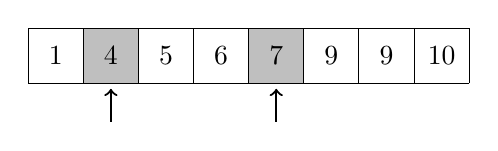
\begin{tikzpicture}[scale=0.7]
\fill[color=lightgray] (1,0) rectangle (2,1);
\fill[color=lightgray] (4,0) rectangle (5,1);
\draw (0,0) grid (8,1);

\node at (0.5,0.5) {$1$};
\node at (1.5,0.5) {$4$};
\node at (2.5,0.5) {$5$};
\node at (3.5,0.5) {$6$};
\node at (4.5,0.5) {$7$};
\node at (5.5,0.5) {$9$};
\node at (6.5,0.5) {$9$};
\node at (7.5,0.5) {$10$};

\draw[thick,->] (1.5,-0.7) -- (1.5,-0.1);
\draw[thick,->] (4.5,-0.7) -- (4.5,-0.1);
\end{tikzpicture}
\end{center}


Després d'això, el punter esquerre torna a moure's un pas cap a la
dreta. El punter dret no es mou i s'ha trobat una solució $5+7=12$.


\begin{center}
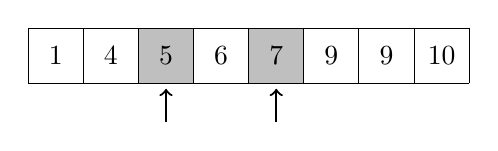
\begin{tikzpicture}[scale=0.7]
\fill[color=lightgray] (2,0) rectangle (3,1);
\fill[color=lightgray] (4,0) rectangle (5,1);
\draw (0,0) grid (8,1);

\node at (0.5,0.5) {$1$};
\node at (1.5,0.5) {$4$};
\node at (2.5,0.5) {$5$};
\node at (3.5,0.5) {$6$};
\node at (4.5,0.5) {$7$};
\node at (5.5,0.5) {$9$};
\node at (6.5,0.5) {$9$};
\node at (7.5,0.5) {$10$};

\draw[thick,->] (2.5,-0.7) -- (2.5,-0.1);
\draw[thick,->] (4.5,-0.7) -- (4.5,-0.1);
\end{tikzpicture}
\end{center}


El temps d'execució de l'algorisme és $O(n \log n)$, perquè primer
ordena el vector en temps $O(n \log n)$, i després els dos punters
mouen $O(n)$ passos.

Tingueu en compte que és possible resoldre el problema d'una altra
manera en temps $O(n \log n)$ fent servir la cerca binària. En aquesta
solució, iterem a través del vector i per a cada valor del vector
intentem trobar un altre valor que produeixi la suma $x$. Això es pot
fer fent $n$ cerques binàries, cadascuna de les quals triga temps
$O(\log n)$.

\index{Problema 3SUMA} Un problema més difícil és el \key{problema 3SUMA},
on es demana trobar \emph{tres} valors del vector la suma dels quals és $x$.
Utilitzant la idea de l'algorisme anterior, aquest problema es pot resoldre
en temps $O(n^2)$\footnote{Durant molt de temps, es va pensar que resoldre el
problema 3SUMA de manera més eficient que en temps $O(n^2) $ no seria
possible. Tanmateix, el 2014, es va veure en \cite{gro14} que no era així.}.
Veus com?

\section{Element menor més propers}

\index{elements menors més propers}

L'anàlisi amortitzada s'utilitza sovint per estimar el nombre
d'operacions realitzades en una estructura de dades. Les operacions
poden estar distribuïdes de manera desigual, de tal forma que la
majoria d'operacions tenen lloc en una fase determinada de
l'algorisme, però el nombre total d'operacions és limitat.

Per exemple, considereu el problema de trobar per a cada element d'un
vector l'\key{element menor més proper}, és a dir, el primer element
menor que l'element original i que el precedeix en el vector. És
possible que no existeixi aquest element, i en aquest cas l'algorisme
hauria d'informar-ho. A continuació veurem com es pot resoldre el
problema de manera eficient mitjançant una estructura de pila.

Recorrem el vector d'esquerra a dreta i mantenim una pila d'elements
del vector. Per cada posició del vector, traiem elements de la pila
fins que l'element superior sigui més petit que l'element actual o la
pila estigui buida. Aleshores, informem que l'element superior és
l'element menor més proper a l'element actual, o si la pila està
buida, l'element no existeix. Finalment, afegim l'element actual a la
pila.

Com a exemple, considereu el vector següent:
\begin{center}
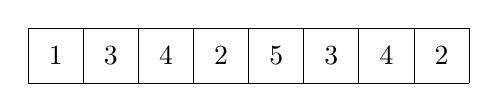
\begin{tikzpicture}[scale=0.7]
\draw (0,0) grid (8,1);

\node at (0.5,0.5) {$1$};
\node at (1.5,0.5) {$3$};
\node at (2.5,0.5) {$4$};
\node at (3.5,0.5) {$2$};
\node at (4.5,0.5) {$5$};
\node at (5.5,0.5) {$3$};
\node at (6.5,0.5) {$4$};
\node at (7.5,0.5) {$2$};
\end{tikzpicture}
\end{center}


En primer lloc, els elements 1, 3 i 4 s'afegeixen a la pila, perquè
cada element és més gran que l'element anterior. Així, l'element menor
més proper de 4 és 3 i l'element menor més proper de 3 és 1.
\begin{center}
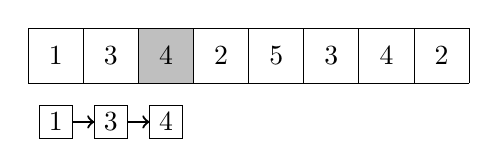
\begin{tikzpicture}[scale=0.7]
\fill[color=lightgray] (2,0) rectangle (3,1);
\draw (0,0) grid (8,1);

\node at (0.5,0.5) {$1$};
\node at (1.5,0.5) {$3$};
\node at (2.5,0.5) {$4$};
\node at (3.5,0.5) {$2$};
\node at (4.5,0.5) {$5$};
\node at (5.5,0.5) {$3$};
\node at (6.5,0.5) {$4$};
\node at (7.5,0.5) {$2$};

\draw (0.2,0.2-1.2) rectangle (0.8,0.8-1.2);
\draw (1.2,0.2-1.2) rectangle (1.8,0.8-1.2);
\draw (2.2,0.2-1.2) rectangle (2.8,0.8-1.2);

\node at (0.5,0.5-1.2) {$1$};
\node at (1.5,0.5-1.2) {$3$};
\node at (2.5,0.5-1.2) {$4$};

\draw[->,thick] (0.8,0.5-1.2) -- (1.2,0.5-1.2);
\draw[->,thick] (1.8,0.5-1.2) -- (2.2,0.5-1.2);
\end{tikzpicture}
\end{center}


El següent element 2 és menor que els dos elements superiors de la
pila. Així, els elements 3 i 4 s'eliminen de la pila i, a continuació,
s'afegeix l'element 2 a la pila. El seu element menor més proper
és 1:
\begin{center}
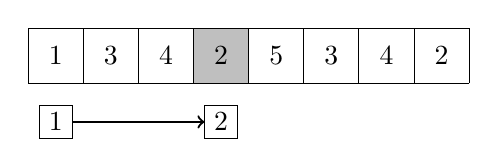
\begin{tikzpicture}[scale=0.7]
\fill[color=lightgray] (3,0) rectangle (4,1);
\draw (0,0) grid (8,1);

\node at (0.5,0.5) {$1$};
\node at (1.5,0.5) {$3$};
\node at (2.5,0.5) {$4$};
\node at (3.5,0.5) {$2$};
\node at (4.5,0.5) {$5$};
\node at (5.5,0.5) {$3$};
\node at (6.5,0.5) {$4$};
\node at (7.5,0.5) {$2$};

\draw (0.2,0.2-1.2) rectangle (0.8,0.8-1.2);
\draw (3.2,0.2-1.2) rectangle (3.8,0.8-1.2);

\node at (0.5,0.5-1.2) {$1$};
\node at (3.5,0.5-1.2) {$2$};

\draw[->,thick] (0.8,0.5-1.2) -- (3.2,0.5-1.2);
\end{tikzpicture}
\end{center}


Aleshores, l'element 5 és més gran que l'element 2, de manera que
s'afegirà a la pila i el seu element menor més proper és 2:
\begin{center}
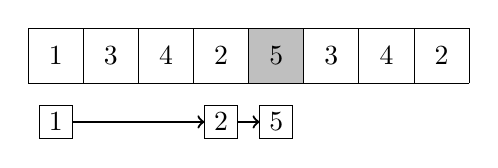
\begin{tikzpicture}[scale=0.7]
\fill[color=lightgray] (4,0) rectangle (5,1);
\draw (0,0) grid (8,1);

\node at (0.5,0.5) {$1$};
\node at (1.5,0.5) {$3$};
\node at (2.5,0.5) {$4$};
\node at (3.5,0.5) {$2$};
\node at (4.5,0.5) {$5$};
\node at (5.5,0.5) {$3$};
\node at (6.5,0.5) {$4$};
\node at (7.5,0.5) {$2$};

\draw (0.2,0.2-1.2) rectangle (0.8,0.8-1.2);
\draw (3.2,0.2-1.2) rectangle (3.8,0.8-1.2);
\draw (4.2,0.2-1.2) rectangle (4.8,0.8-1.2);

\node at (0.5,0.5-1.2) {$1$};
\node at (3.5,0.5-1.2) {$2$};
\node at (4.5,0.5-1.2) {$5$};

\draw[->,thick] (0.8,0.5-1.2) -- (3.2,0.5-1.2);
\draw[->,thick] (3.8,0.5-1.2) -- (4.2,0.5-1.2);
\end{tikzpicture}
\end{center}


Després d'això, l'element 5 s'elimina de la pila i els elements 3 i 4
s'afegeixen a la pila:
\begin{center}
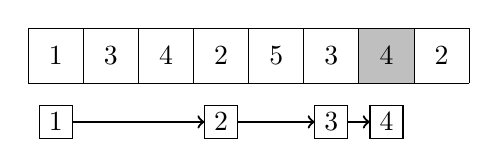
\begin{tikzpicture}[scale=0.7]
\fill[color=lightgray] (6,0) rectangle (7,1);
\draw (0,0) grid (8,1);

\node at (0.5,0.5) {$1$};
\node at (1.5,0.5) {$3$};
\node at (2.5,0.5) {$4$};
\node at (3.5,0.5) {$2$};
\node at (4.5,0.5) {$5$};
\node at (5.5,0.5) {$3$};
\node at (6.5,0.5) {$4$};
\node at (7.5,0.5) {$2$};

\draw (0.2,0.2-1.2) rectangle (0.8,0.8-1.2);
\draw (3.2,0.2-1.2) rectangle (3.8,0.8-1.2);
\draw (5.2,0.2-1.2) rectangle (5.8,0.8-1.2);
\draw (6.2,0.2-1.2) rectangle (6.8,0.8-1.2);

\node at (0.5,0.5-1.2) {$1$};
\node at (3.5,0.5-1.2) {$2$};
\node at (5.5,0.5-1.2) {$3$};
\node at (6.5,0.5-1.2) {$4$};

\draw[->,thick] (0.8,0.5-1.2) -- (3.2,0.5-1.2);
\draw[->,thick] (3.8,0.5-1.2) -- (5.2,0.5-1.2);
\draw[->,thick] (5.8,0.5-1.2) -- (6.2,0.5-1.2);
\end{tikzpicture}
\end{center}


Finalment, tots els elements excepte l'1 s'eliminen de la pila i
l'últim element 2 s'afegeix a la pila:


\begin{center}
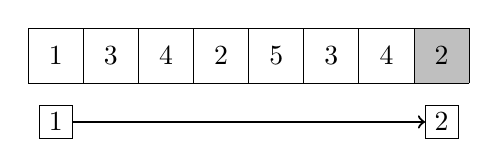
\begin{tikzpicture}[scale=0.7]
\fill[color=lightgray] (7,0) rectangle (8,1);
\draw (0,0) grid (8,1);

\node at (0.5,0.5) {$1$};
\node at (1.5,0.5) {$3$};
\node at (2.5,0.5) {$4$};
\node at (3.5,0.5) {$2$};
\node at (4.5,0.5) {$5$};
\node at (5.5,0.5) {$3$};
\node at (6.5,0.5) {$4$};
\node at (7.5,0.5) {$2$};

\draw (0.2,0.2-1.2) rectangle (0.8,0.8-1.2);
\draw (7.2,0.2-1.2) rectangle (7.8,0.8-1.2);

\node at (0.5,0.5-1.2) {$1$};
\node at (7.5,0.5-1.2) {$2$};

\draw[->,thick] (0.8,0.5-1.2) -- (7.2,0.5-1.2);
\end{tikzpicture}
\end{center}


L'eficiència de l'algorisme depèn del nombre total d'operacions fets a
la pila. Si l'element actual és més gran que l'element superior de la
pila, s'afegeix directament a la pila, la qual cosa és
eficient. Tanmateix, de vegades la pila pot contenir diversos elements
més grans i es necessita temps per eliminar-los. Tot i així, cada
element s'afegeix \emph{exactament una vegada} a la pila i s'elimina
\emph{com a màxim una vegada} de la pila. Així, cada element provoca
$O(1)$ operacions de pila, i l'algorisme funciona en temps $O(n)$.

\section{Mínim de finestra lliscant}

\index{Mínim de finestra lliscant} \index{finestra lliscant}

Una finestra lliscant (\key{sliding window}) és un subvector de mida
constant que es mou d'esquerra a dreta a través del vector. A cada
posici de la finestra, volem calcular una certa informació sobre els
elements dins de la finestra. En aquesta secció, ens centrem en el
problema de mantenir el \key{mínim de la finestra}, és a dir, el valor
més petit dins de cada finestra.

El mínim de la finestra lliscant es pot calcular fent servir una idea
semblant a la dels elements menors més propers. Mantenim una cua on
cada element és més gran que l'element anterior, i el primer element
sempre es correspon amb l'element mínim de la finestra. Després de
cada moviment de la finestra, treiem elements del final de la cua fins
que l'últim element de la cua sigui més petit que l'element de la
nova finestra, o la cua quedi buida. També eliminem el primer element
de la cua si ja no està dins de la finestra. Finalment, afegim l'element
de la nova finestra al final de la cua.

Com a exemple, considereu el vector següent:


\begin{center}
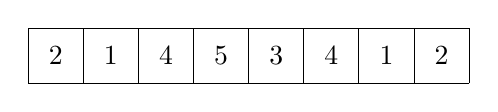
\begin{tikzpicture}[scale=0.7]
\draw (0,0) grid (8,1);

\node at (0.5,0.5) {$2$};
\node at (1.5,0.5) {$1$};
\node at (2.5,0.5) {$4$};
\node at (3.5,0.5) {$5$};
\node at (4.5,0.5) {$3$};
\node at (5.5,0.5) {$4$};
\node at (6.5,0.5) {$1$};
\node at (7.5,0.5) {$2$};
\end{tikzpicture}
\end{center}


Suposem que la mida de la finestra lliscant és 4. A la primera posició
de la finestra, el valor més petit és 1:
\begin{center}
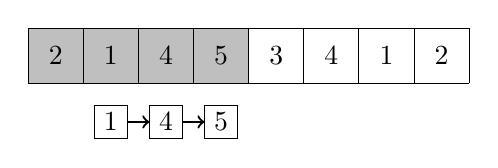
\begin{tikzpicture}[scale=0.7]
\fill[color=lightgray] (0,0) rectangle (4,1);
\draw (0,0) grid (8,1);

\node at (0.5,0.5) {$2$};
\node at (1.5,0.5) {$1$};
\node at (2.5,0.5) {$4$};
\node at (3.5,0.5) {$5$};
\node at (4.5,0.5) {$3$};
\node at (5.5,0.5) {$4$};
\node at (6.5,0.5) {$1$};
\node at (7.5,0.5) {$2$};

\draw (1.2,0.2-1.2) rectangle (1.8,0.8-1.2);
\draw (2.2,0.2-1.2) rectangle (2.8,0.8-1.2);
\draw (3.2,0.2-1.2) rectangle (3.8,0.8-1.2);

\node at (1.5,0.5-1.2) {$1$};
\node at (2.5,0.5-1.2) {$4$};
\node at (3.5,0.5-1.2) {$5$};

\draw[->,thick] (1.8,0.5-1.2) -- (2.2,0.5-1.2);
\draw[->,thick] (2.8,0.5-1.2) -- (3.2,0.5-1.2);
\end{tikzpicture}
\end{center}


Aleshores, la finestra es mou un pas cap a la dreta. El nou element 3
és més petit que els elements 4 i 5 de la cua, de manera que els
elements 4 i 5 s'eliminen de la cua i l'element 3 s'afegeix a la
cua. El valor més petit segueix sent 1.
\begin{center}
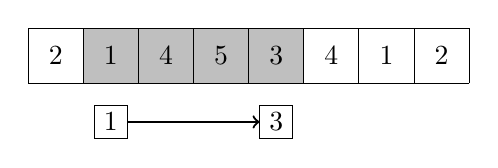
\begin{tikzpicture}[scale=0.7]
\fill[color=lightgray] (1,0) rectangle (5,1);
\draw (0,0) grid (8,1);

\node at (0.5,0.5) {$2$};
\node at (1.5,0.5) {$1$};
\node at (2.5,0.5) {$4$};
\node at (3.5,0.5) {$5$};
\node at (4.5,0.5) {$3$};
\node at (5.5,0.5) {$4$};
\node at (6.5,0.5) {$1$};
\node at (7.5,0.5) {$2$};

\draw (1.2,0.2-1.2) rectangle (1.8,0.8-1.2);
\draw (4.2,0.2-1.2) rectangle (4.8,0.8-1.2);

\node at (1.5,0.5-1.2) {$1$};
\node at (4.5,0.5-1.2) {$3$};

\draw[->,thick] (1.8,0.5-1.2) -- (4.2,0.5-1.2);
\end{tikzpicture}
\end{center}


Després d'això, la finestra es mou de nou i l'element més petit 1 ja
no pertany a la finestra. Així, s'elimina de la cua i el valor més
petit és ara 3. També s'afegeix el nou element 4 a la cua.
\begin{center}
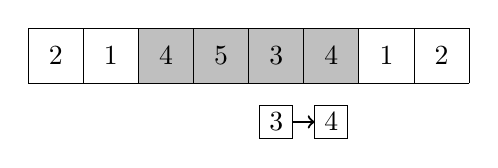
\begin{tikzpicture}[scale=0.7]
\fill[color=lightgray] (2,0) rectangle (6,1);
\draw (0,0) grid (8,1);

\node at (0.5,0.5) {$2$};
\node at (1.5,0.5) {$1$};
\node at (2.5,0.5) {$4$};
\node at (3.5,0.5) {$5$};
\node at (4.5,0.5) {$3$};
\node at (5.5,0.5) {$4$};
\node at (6.5,0.5) {$1$};
\node at (7.5,0.5) {$2$};

\draw (4.2,0.2-1.2) rectangle (4.8,0.8-1.2);
\draw (5.2,0.2-1.2) rectangle (5.8,0.8-1.2);

\node at (4.5,0.5-1.2) {$3$};
\node at (5.5,0.5-1.2) {$4$};

\draw[->,thick] (4.8,0.5-1.2) -- (5.2,0.5-1.2);
\end{tikzpicture}
\end{center}


El següent element nou 1 és més petit que tots els elements de la
cua. Així, tots els elements s'eliminen de la cua i aquesta només
contindrà l'element 1:
\begin{center}
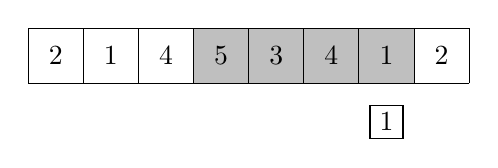
\begin{tikzpicture}[scale=0.7]
\fill[color=lightgray] (3,0) rectangle (7,1);
\draw (0,0) grid (8,1);

\node at (0.5,0.5) {$2$};
\node at (1.5,0.5) {$1$};
\node at (2.5,0.5) {$4$};
\node at (3.5,0.5) {$5$};
\node at (4.5,0.5) {$3$};
\node at (5.5,0.5) {$4$};
\node at (6.5,0.5) {$1$};
\node at (7.5,0.5) {$2$};

\draw (6.2,0.2-1.2) rectangle (6.8,0.8-1.2);

\node at (6.5,0.5-1.2) {$1$};
\end{tikzpicture}
\end{center}


Finalment la finestra arriba a la seva última posició. L'element 2
s'afegeix a la cua, però el valor més petit dins de la finestra
segueix sent 1.
\begin{center}
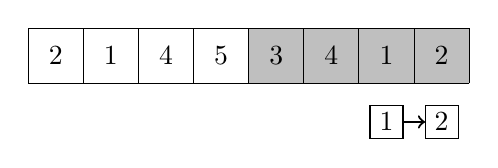
\begin{tikzpicture}[scale=0.7]
\fill[color=lightgray] (4,0) rectangle (8,1);
\draw (0,0) grid (8,1);

\node at (0.5,0.5) {$2$};
\node at (1.5,0.5) {$1$};
\node at (2.5,0.5) {$4$};
\node at (3.5,0.5) {$5$};
\node at (4.5,0.5) {$3$};
\node at (5.5,0.5) {$4$};
\node at (6.5,0.5) {$1$};
\node at (7.5,0.5) {$2$};

\draw (6.2,0.2-1.2) rectangle (6.8,0.8-1.2);
\draw (7.2,0.2-1.2) rectangle (7.8,0.8-1.2);

\node at (6.5,0.5-1.2) {$1$};
\node at (7.5,0.5-1.2) {$2$};

\draw[->,thick] (6.8,0.5-1.2) -- (7.2,0.5-1.2);
\end{tikzpicture}
\end{center}


Com que cada element del vector s'afegeix a la cua exactament una
vegada i s'elimina de la cua com a màxim una vegada, l'algorisme
funciona en temps $O(n)$.
